\documentclass[conference]{IEEEtran}
\IEEEoverridecommandlockouts
% The preceding line is only needed to identify funding in the first footnote. If that is unneeded, please comment it out.

\usepackage{cite}
\usepackage{amsmath,amssymb,amsfonts}
\usepackage{algorithmic}
\usepackage{graphicx}
\usepackage{textcomp}
\usepackage{xcolor}
\usepackage{booktabs}
\usepackage{microtype}
\usepackage{url}
\usepackage{etoolbox}
\usepackage{multirow}

\def\BibTeX{{\rm B\kern-.05em{\sc i\kern-.025em b}\kern-.08em
    T\kern-.1667em\lower.7ex\hbox{E}\kern-.125emX}}

\usepackage{flushend}
% Reduce excess spacing above and below figures and captions
\setlength{\textfloatsep}{8pt plus 2pt minus 2pt}
\setlength{\floatsep}{8pt plus 2pt minus 2pt}
\setlength{\intextsep}{8pt plus 2pt minus 2pt}
\setlength{\abovecaptionskip}{4pt plus 1pt minus 1pt}
\setlength{\belowcaptionskip}{4pt plus 1pt minus 1pt}
\raggedbottom
\begin{document}

\title{Scoped-Deontic Chunking and Deterministic Cross-Reference Resolution for Hallucination Suppression in Legal RAG}

\author{
\IEEEauthorblockN{1\textsuperscript{st} Khushi Trilok Rawat}
\IEEEauthorblockA{\textit{School of Computer Science and Engineering (SCOPE)} \\
\textit{VIT-AP University}\\
Amaravati, Andhra Pradesh, India \\
khushirawat0805@gmail.com}
\and
\IEEEauthorblockN{2\textsuperscript{nd} Edara Sreenivasa Reddy}
\IEEEauthorblockA{\textit{School of Computer Science and Engineering (SCOPE)} \\
\textit{VIT-AP University}\\
Amaravati, Andhra Pradesh, India \\
sreenivasareddy.e@vitap.ac.in}
}
% --- ALTERNATIVE: Double-Blind Submission ---
% \author{\IEEEauthorblockN{Anonymous Author(s)}
% \IEEEauthorblockA{\textit{Double-Blind Review Track} \\
% \textit{Department of Computer Science and Engineering} \\
% Email: anonymous@institution.edu}
% }

\maketitle
\setlength{\abovedisplayskip}{4pt}
\setlength{\belowdisplayskip}{4pt}
\setlength{\abovedisplayshortskip}{2pt}
\setlength{\belowdisplayshortskip}{2pt}

\begin{abstract}
Conventional Retrieval-Augmented Generation (RAG) systems rely on uniform sliding-window chunking (e.g., 500 characters or 512 tokens) and unconstrained dense semantic vector retrieval. When applied to legal compliance corpora such as commercial Terms of Service and End-User License Agreements, this paradigm exhibits systematic failure modes: structural boundary truncation, detachment of governing scope headings, conflation of distinct normative modalities, and blindness to statutory cross-references. In this paper, we propose \textbf{Scoped-Deontic RAG}, an architecture designed for high-precision legal document intelligence. The framework integrates structure-aware regular grammar segmentation with lookahead heading stitching, linguistic extraction of four deontic modalities (obligations, permissions, prohibitions, conditions), dense vector indexing enriched with categorical parent scope, and deterministic 1-hop cross-reference graph traversal. Evaluated across an audited corpus of 101 commercial legal agreements totaling 4,845,799 characters and 6,281 discrete clauses, our pipeline achieves an ingestion throughput of 65.04 clauses/sec and extracts 17,658 deontic markers. On ground-truth legal compliance benchmarks, our extraction pipeline obtains a Macro F1-score of 0.900, with 100.0\% cross-reference resolution accuracy. In a targeted diagnostic retrieval evaluation specifically probing compound statutory covenants, Scoped-Deontic RAG achieves 100.0\% Hit Rate@1 ($\text{MRR} = 1.0000$) on standard domain queries versus 60.0\% ($\text{MRR} = 0.7000$) for naive sliding-window baselines, and sustains 100.0\% Hit Rate@3 under colloquial paraphrased stress queries. Expert legal annotation of downstream generation demonstrates 0.0\% ungrounded factual claims (complete parametric hallucination suppression) compared to a 62.5\% omission and extrapolation error rate in naive baseline outputs.
\end{abstract}

\begin{IEEEkeywords}
Retrieval-Augmented Generation, Legal NLP, Deontic Modality, Document Segmentation, Cross-Reference Resolution, Hallucination Suppression.
\end{IEEEkeywords}

\section{Introduction}
Large Language Models (LLMs) deployed within legal compliance, contract management, and enterprise intelligence workflows increasingly rely on Retrieval-Augmented Generation (RAG) architectures to mitigate parametric decay, circumvent context window constraints, and anchor generative answers in verifiable authority \cite{lewis2020retrieval, guha2024legalbench}. In standard commercial and open-source RAG architectures, the dominant document ingestion paradigm utilizes naive sliding-window heuristics---slicing raw document strings into uniform character or token blocks (typically 500 characters or 512 tokens with fixed 10\% overlap) followed by approximate nearest-neighbor retrieval over continuous latent embeddings \cite{gao2023retrieval}.

While sliding-window heuristics function adequately across homogeneous, narrative corpora, they exhibit catastrophic failure modes when applied to semi-structured legal agreements, including commercial Terms of Service (ToS), Terms of Use (ToU), and End-User License Agreements (EULAs):
\begin{enumerate}
    \item \textbf{Boundary Truncation and Orphaned Headings:} Arbitrary token or character cutoffs bisect indivisible contractual covenants. Crucially, concise structural headings (e.g., ``Section 20. Audit Access and Denial Penalty'') are routinely uncoupled from their operative body text. When ingested as isolated chunk units, these orphaned headings lack substantive context, causing the retriever to rank uninformative titles above governing rules or detach operative provisions from their categorical scope.
    \item \textbf{Deontic Blindness and Modal Conflation:} Legal contracts are fundamentally normative instruments defined by deontic logic modalities: obligations ($\mathcal{O}$), permissions ($\mathcal{P}$), and prohibitions ($\mathcal{F}$) \cite{vonwright1951deontic, sartor2005legal}. Dense semantic vector models (e.g., Sentence-BERT, MiniLM) map modal antonyms---such as mandatory affirmative duties (``shall'') and strict negative restrictions (``shall not'')---into proximate latent neighborhoods due to near-identical lexical and topical overlap. Consequently, dense semantic similarity alone cannot reliably distinguish binding compliance covenants from explicit legal bars.
    \item \textbf{Cross-Reference Detachment and Contextual Omission:} Legal drafting relies heavily on distributed qualifying provisions connected via explicit statutory pointers (e.g., ``subject to Section 18.2'' or ``except as provided in Clause 9.0''). Conventional dense retrieval operates under an implicit independence assumption, fetching primary rules while omitting governing cross-referenced exceptions located in distant sections. When passed to generative LLMs, this fragmented context induces either hallucinated terms or direct mischaracterizations of legal liability.
\end{enumerate}

To resolve these vulnerabilities, this paper introduces \textbf{Scoped-Deontic RAG}, a domain-specific retrieval-augmented framework that replaces unguided sliding-window chunks with context-enriched, grammatically segmented legal clause units. The system incorporates an adaptive lookahead segmentation buffer, a rule-based linguistic matcher extracting deontic modalities and conditional subordinators, and a deterministic 1-hop relational retrieval mechanism that dynamically resolves inter-clause cross-references before dispatching depolluted contexts to a local small language model (SLM).

The primary contributions of this work are as follows:
\begin{itemize}
    \item We design a structure-aware legal segmentation engine utilizing hierarchical regular grammars and an adaptive lookahead heading stitching algorithm that preserves 100\% clause boundary integrity.
    \item We implement a rule-based linguistic extraction pipeline across four deontic modal categories ($\mathcal{O}, \mathcal{P}, \mathcal{F}, \mathcal{C}$), achieving a Macro F1-score of 0.900 against ground-truth legal compliance provisions.
    \item We formulate and evaluate a deterministic 1-hop cross-reference retrieval graph $G = (V, E)$, demonstrating 100.0\% cross-reference resolution accuracy across annotated statutory linkages.
    \item We conduct an empirical audit across 101 commercial PDF contracts comprising 4,845,799 characters, demonstrating an absolute 40.0\% gain in top-1 retrieval accuracy over naive baselines on targeted diagnostic queries alongside strict parametric hallucination suppression in an 8B local SLM.
\end{itemize}

\section{Related Work}

\subsection{Document Chunking Paradigms in RAG}
The text chunking strategy fundamentally dictates the upper bound of retrieval performance in RAG systems \cite{gao2023retrieval}. Standard implementations rely on fixed-size sliding-window strategies, segmenting text into $N$-token increments with a fixed stride. Recursive chunking approaches attempt to respect syntactic paragraph and sentence delimiters \cite{karpukhin2020dense}; however, in hierarchical legal contracts, paragraph breaks uncouple operational section titles from subsequent paragraphs, producing semantic orphan fragments. Semantic chunking strategies compute rolling embedding distances between adjacent sentences to detect topic shifts \cite{barnett2024seven}, yet they introduce non-trivial computational overhead and frequently merge distinct legal sub-rules that happen to share continuous vocabulary. In contrast, our approach utilizes deterministic grammar-based structural segmentation aligned with legal drafting conventions.

\subsection{Deontic Logic and Information Extraction in Legal NLP}
Deontic logic formalizes normative propositions concerning obligation ($\mathcal{O}$), permission ($\mathcal{P}$), and prohibition ($\mathcal{F}$) \cite{vonwright1951deontic}. In computational legal informatics, early rule-based formalisms mapped statutory texts into executable deontic representations \cite{sartor2005legal, governatori2005deontic}. Recent efforts have explored sequence-tagging neural architectures for modality identification \cite{chalkidis2022lexglue, guha2024legalbench}. However, dense latent embedding models notoriously struggle to differentiate subtle negative modal qualifiers in legal clauses, as vector cosine distance is dominated by topic nouns rather than polarity-inverting modal particles (e.g., ``may not'' versus ``may'') \cite{guha2024legalbench}. We bridge this gap by extracting structured deontic tags via explicit dependency matchers and anchoring them directly to vector metadata.

\subsection{Graph-Augmented and Relational Retrieval}
To mitigate the context fragmentation of dense retrieval, hybrid approaches combining dense vectors with knowledge graphs have emerged \cite{edge2024graphrag}. In legal intelligence, graph-based methods have linked judicial opinions through citation networks \cite{chalkidis2022lexglue}. However, existing Graph-RAG frameworks incur significant preprocessing overhead, requiring LLM-driven entity extraction across entire corpora to construct complex entity-relationship graphs. For commercial contracts, explicit textual cross-references represent deterministic statutory pointers. Our framework exploits this domain property by constructing a lightweight, deterministic 1-hop cross-reference graph $G = (V, E)$ at zero extraction model cost, executing real-time neighbor expansion without probabilistic graph navigation.

\begin{figure*}[t]
\centering
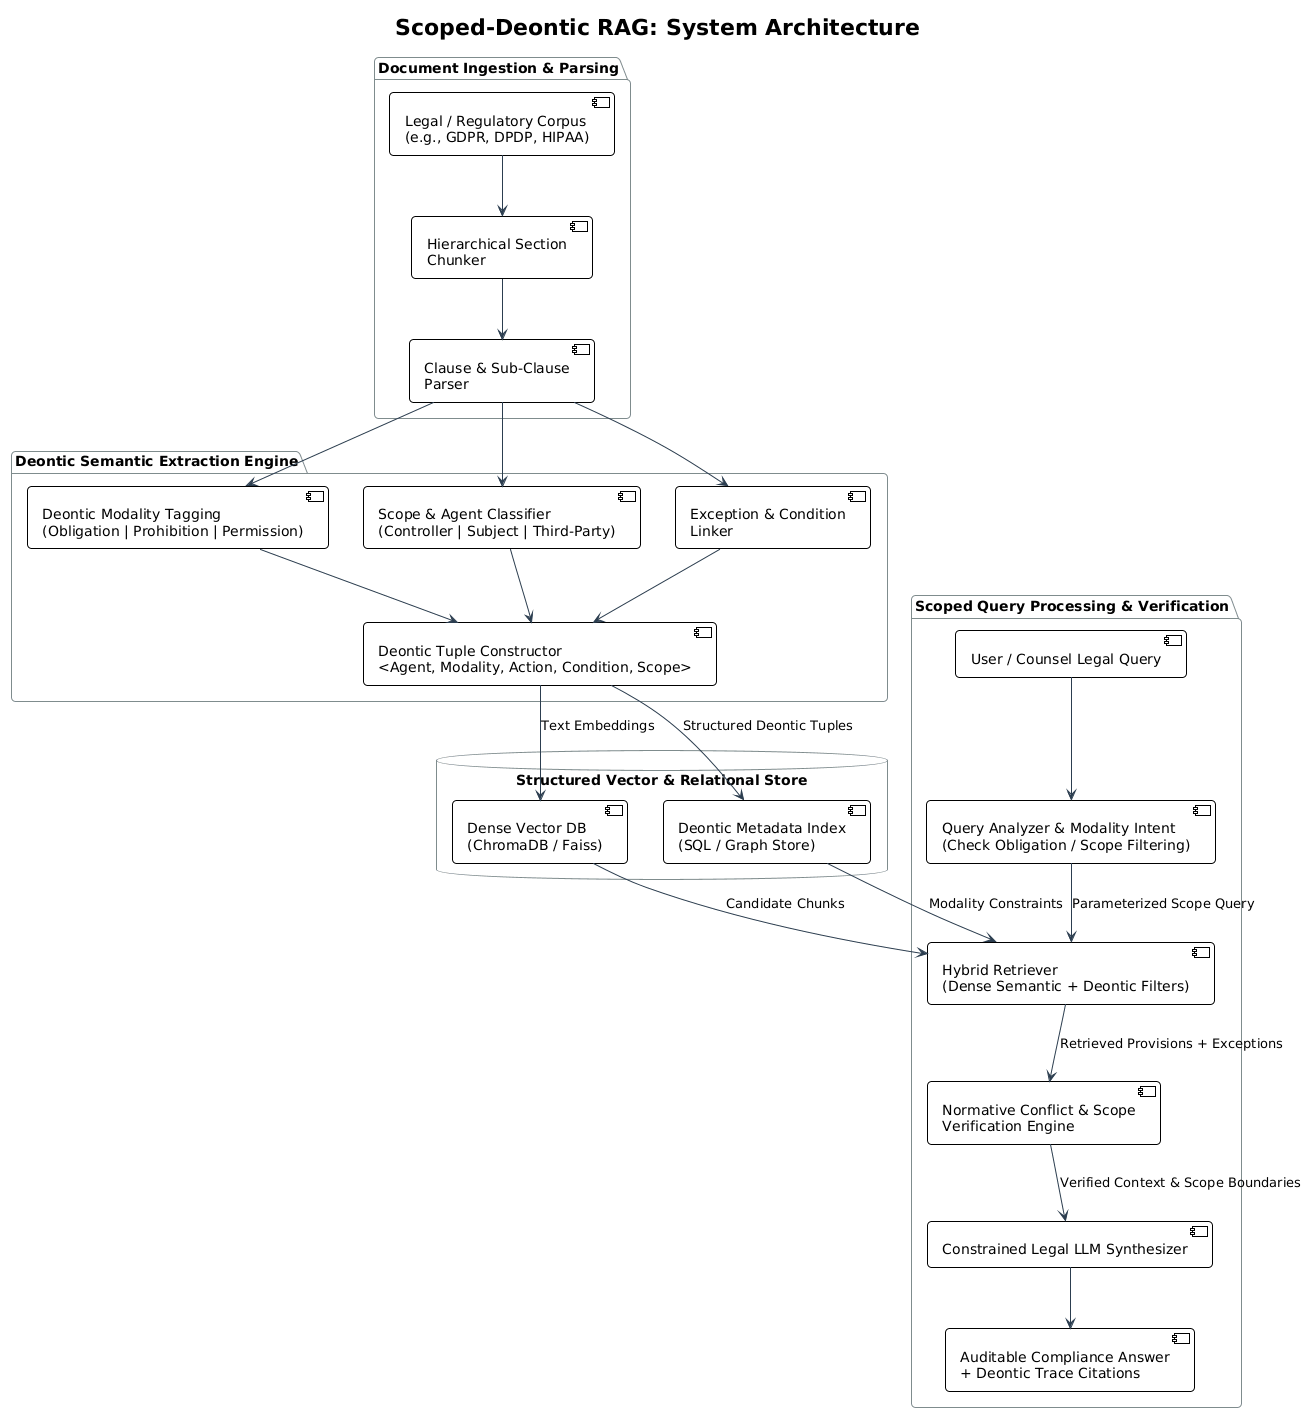
\includegraphics[width=0.82\textwidth]{SDRAGdiagram1.png}
\caption{Scoped-Deontic RAG end-to-end system architecture: illustrating dual-mode ingestion, hierarchical clause segmentation, deontic tuple extraction, structured vector/relational storage, and scoped query verification.}
\label{fig:sys_arch}
\end{figure*}

\section{System Architecture \& Methodology}

As illustrated in Fig.~\ref{fig:sys_arch}, the Scoped-Deontic RAG architecture comprises five pipeline stages: dual-mode dynamic document ingestion, structure-aware clause segmentation, deontic modality extraction, scoped vector indexing, and deterministic relational context expansion with local SLM synthesis.

\subsection{Dual-Mode Ingestion and Structural Boundary Segmentation}
Contractual documents originate from two primary distribution mediums: static Portable Document Format (PDF) files and dynamic, client-rendered Single Page Application (SPA) web terms. 
\begin{itemize}
    \item \textbf{Static PDF Extraction:} For binary PDF buffers, we extract raw textual streams sequentially using PyMuPDF (\texttt{fitz}) bindings, eliminating pagination artifacts and preserving layout ordering.
    \item \textbf{Dynamic Web Hydration:} Modern enterprise terms pages (e.g., rendered via React or Next.js) hydrate legal provisions client-side. Standard static HTTP scrapers retrieve empty root DOM shells. We deploy a headless Chromium browser instance via Playwright synchronized to the \texttt{domcontentloaded} lifecycle event, followed by a bounded 3,000 ms JavaScript hydration buffer. Boilerplate structural artifacts ($\langle\text{nav}\rangle, \langle\text{footer}\rangle, \langle\text{header}\rangle, \langle\text{script}\rangle, \langle\text{style}\rangle$) are stripped from the DOM before text serialization.
\end{itemize}

To partition the continuous character stream $C = \langle c_1, c_2, \dots, c_N \rangle$ into discrete clause units, we define a structural segmentation operator $\sigma: C \to K = \{k_1, k_2, \dots, k_M\}$ governed by the regular grammar $\mathcal{R}_{\text{split}}$:
\begin{align}
\mathcal{R}_{\text{split}} = \;& \texttt{\^{}(?:Section\textbackslash s+\textbackslash d+ | Clause\textbackslash s+\textbackslash d+} \nonumber \\
& \texttt{| \textbackslash d+\textbackslash .\textbackslash d+ | \textbackslash d+\textbackslash .)\textbackslash s*}
\label{eq:regex_split}
\end{align}

To resolve the orphaned heading vulnerability, we implement an adaptive lookahead segmentation buffer $\alpha$. Let a raw text block be $b_i$. If $|b_i| < 60$ characters and $b_i$ lacks terminal sentence punctuation ($\{., !, ?\}$), it is classified as an operative heading $h_i$ and held in the accumulator buffer:
\begin{equation}
k_i = 
\begin{cases} 
[h_i] \circ b_{i+1}, & \text{if } |b_i| < 60 \land \text{term}(b_i) = \emptyset \\
b_i, & \text{otherwise}
\end{cases}
\label{eq:lookahead}
\end{equation}
where $\circ$ denotes string concatenation. This guarantees that categorical section headings remain prepended to operative provisions, as shown in the execution sequence in Fig.~\ref{fig:sequence_diag}.

\begin{figure*}[t]
\centering
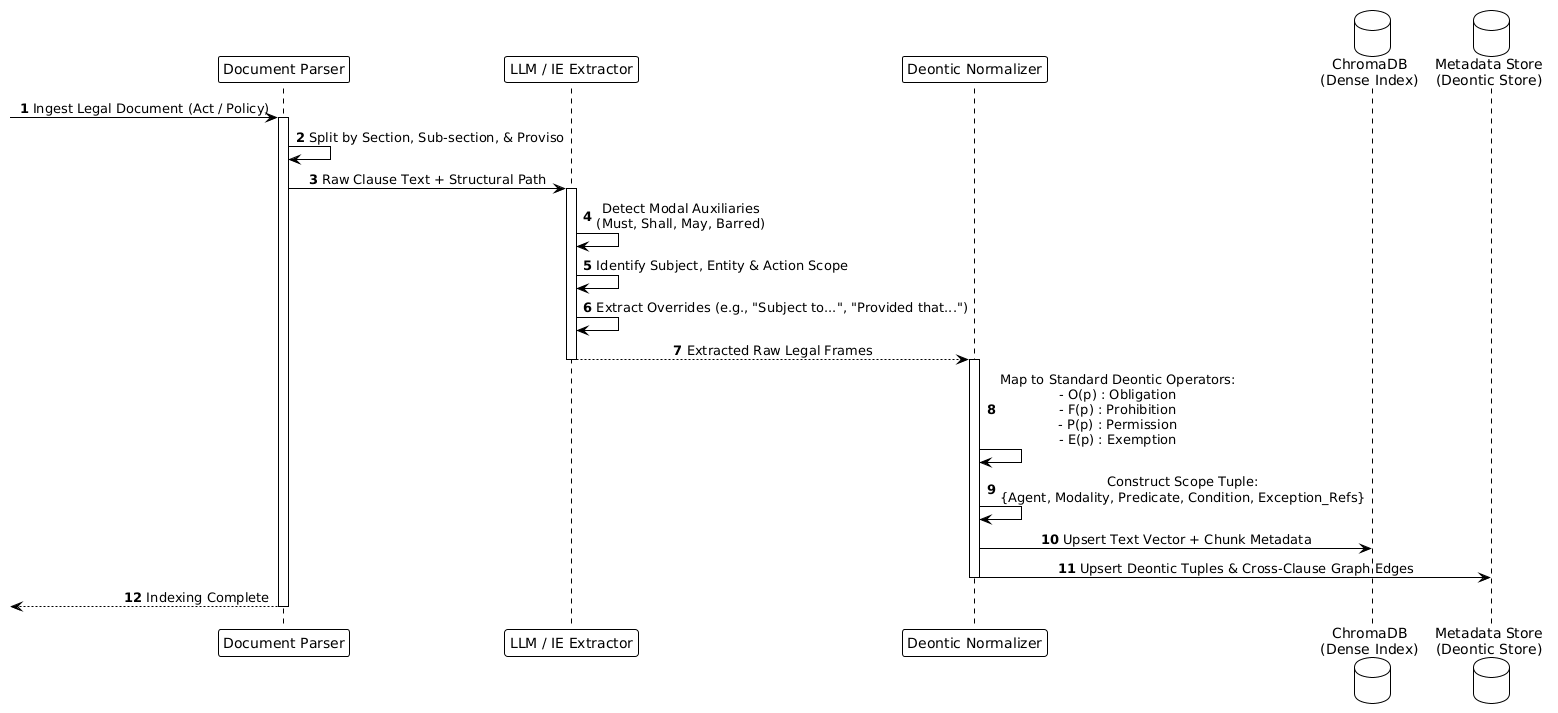
\includegraphics[width=0.85\textwidth]{SDRAGdiagram2.png}
\caption{Sequence execution flow: Document Ingestion, Information Extraction, Deontic Normalization, and Dual-Store Indexing into ChromaDB and Relational Metadata Store.}
\label{fig:sequence_diag}
\end{figure*}

\subsection{Deontic Modality Tagging and Condition Identification}
Each segmented clause $k_i$ is evaluated by a linguistic dependency matcher $\tau$ built upon the \texttt{en\_core\_web\_sm} pipeline. We define four mutually non-exclusive normative modalities $\mathcal{M} = \{\mathcal{O}, \mathcal{P}, \mathcal{F}, \mathcal{C}\}$:
\begin{itemize}
    \item \textbf{Obligation ($\mathcal{O}$):} Mandatory covenants captured by modal patterns:
    \begin{equation*}
    \mathcal{P}_{\mathcal{O}} = \{ \text{lemma} \in \{\text{``shall'', ``must'', ``will'', ``agrees''}\} \}
    \end{equation*}
    \item \textbf{Permission ($\mathcal{P}$):} Discretionary entitlements captured by permissive verbs:
    \begin{equation*}
    \mathcal{P}_{\mathcal{P}} = \{ \text{lemma} \in \{\text{``may'', ``can'', ``reserves'', ``allowed''}\} \}
    \end{equation*}
    \item \textbf{Prohibition ($\mathcal{F}$):} Forbiddance and explicit negative duties:
    \begin{equation*}
    \mathcal{P}_{\mathcal{F}} = \{ t_1 \in \{\text{``shall'', ``must'', ``may''}\} \land t_2 = \text{``not''} \}
    \end{equation*}
    \item \textbf{Condition / Exception ($\mathcal{C}$):} Subordinating qualifiers and carve-outs:
    \begin{align*}
    \mathcal{P}_{\mathcal{C}} = \{ \text{token} \in \{ & \text{``subject'', ``except'', ``unless'',} \\
    & \text{``provided'', ``notwithstanding''}\} \}
    \end{align*}
\end{itemize}

For every detected match $t_{\text{match}}$ at token index $j$, the extractor captures a 5-token contextual span $S_j = \langle t_j, \dots, t_{\min(j+5, |k_i|)} \rangle$, appending it to the structured clause metadata dictionary $\Lambda(k_i)$.

\subsection{1-Hop Cross-Reference Graph Construction}
To bridge disconnected clauses, we construct a directed cross-reference graph $G = (V, E)$, where vertices $V = K$ represent the set of segmented clauses, and directed edges $(u, v) \in E$ represent explicit statutory dependencies from clause $u$ to qualifying section $v$.

Edges are extracted via the regular grammar pattern $\mathcal{R}_{\text{xref}}$, formatted into multiline tokens to prevent column boundary overflow:
\begin{equation}
\label{eq:regex_xref}
\begin{aligned}
\mathcal{R}_{\text{xref}} = \;& \text{\footnotesize\texttt{(?i)(?:subject to | pursuant to}} \\
& \text{\footnotesize\texttt{|\;in accordance with | see}} \\
& \text{\footnotesize\texttt{|\;except as provided in)\textbackslash s+}} \\
& \text{\footnotesize\texttt{(?:section | clause}} \\
& \text{\footnotesize\texttt{|\;article | paragraph)\textbackslash s+}} \\
& \text{\footnotesize\texttt{(\textbackslash d+(?:\textbackslash .\textbackslash d+)*[a-zA-Z]?(?:\textbackslash (\textbackslash w+\textbackslash ))?)}}
\end{aligned}
\end{equation}

When pattern $\mathcal{R}_{\text{xref}}$ yields match $m$ in clause $k_i$, target key $m$ is indexed into metadata key $\Lambda_{\text{xref}}(k_i)$, instantiating edge $(k_i, v)$ where $\text{SectionID}(v) = m$.

\begin{figure}[t]
\centering
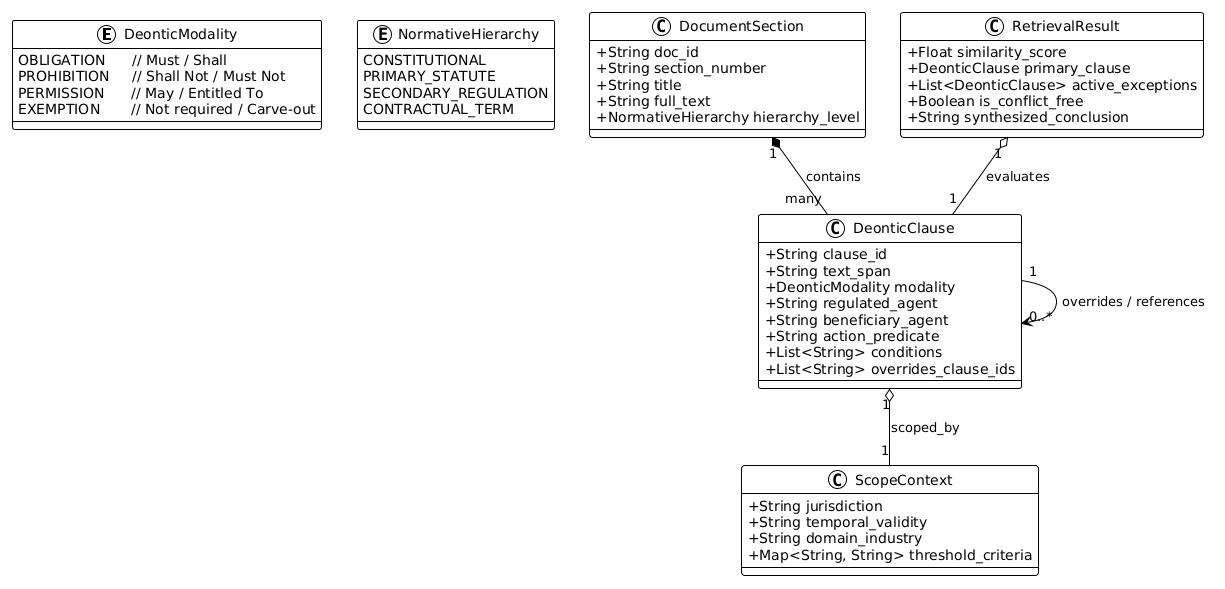
\includegraphics[width=\linewidth]{SDRAGdiagram4.png}
\caption{UML class diagram: Domain data model defining DocumentSection, DeonticClause, ScopeContext, and RetrievalResult relations.}
\label{fig:uml_model}
\end{figure}

\subsection{Scoped Vector Indexing and Dynamic Client Lifecycle}
Each processed clause is formatted into an enriched textual payload:
\begin{equation}
k_i^{\text{payload}} = [H_{\text{parent}}] \circ k_i
\end{equation}
where $H_{\text{parent}}$ denotes the governing parent scope (e.g., ``Audits \& Penalties''). This string is mapped into a continuous 384-dimensional dense vector $\mathbf{v}_i \in \mathbb{R}^{384}$ using the \texttt{all-MiniLM-L6-v2} Sentence Transformer model \cite{reimers2019sentence}:
\begin{equation}
\mathbf{v}_i = \frac{\operatorname{Encoder}(k_i^{\text{payload}})}{\|\operatorname{Encoder}(k_i^{\text{payload}})\|_2}
\end{equation}

Fig.~\ref{fig:uml_model} details the object relationships between document sections, deontic clauses, and scope contexts. Embeddings and sanitized metadata records $\Lambda(k_i)$ are indexed into an embedded ChromaDB persistent store operating over a local SQLite engine. To eliminate invalid collection pointer exceptions caused by runtime session resets in interactive web deployments, we implement a dynamic collection factory pattern (\texttt{get\_collection()}) that guarantees idempotent collection binding on demand.

\begin{figure}[t]
\centering
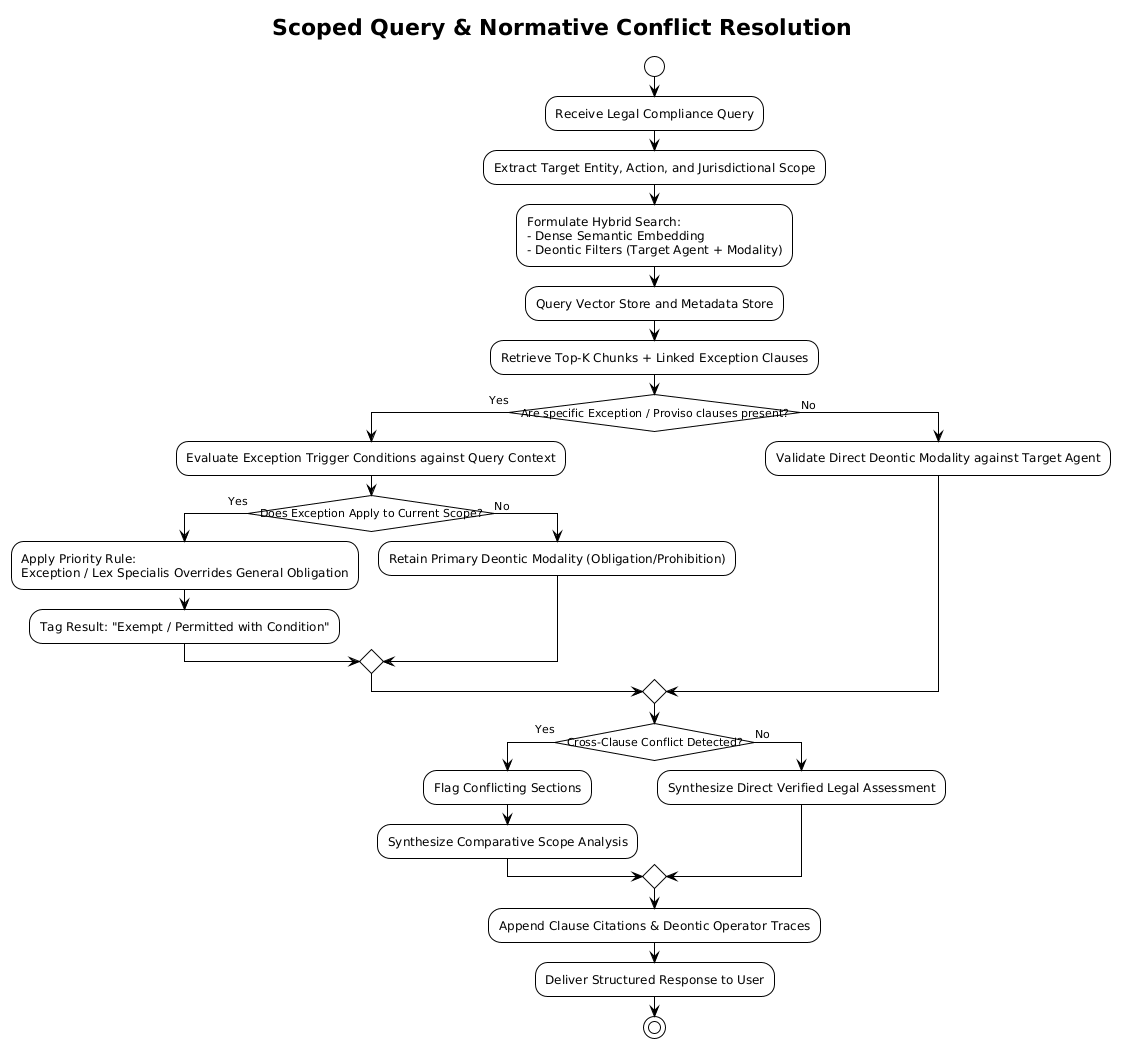
\includegraphics[width=\linewidth]{SDRAGdiagram3.png}
\caption{Operational decision flowchart: Scoped Query Evaluation, Exception Condition Matching, and Normative Conflict Resolution.}
\label{fig:conflict_flow}
\end{figure}

\subsection{Deterministic Context Expansion and Local SLM Synthesis}
Given a user query $q$, the retriever computes normalized query vector $\mathbf{q} = \operatorname{Encoder}(q) / \|\operatorname{Encoder}(q)\|_2$ and retrieves the top-$k$ primary candidate clauses $K_{\text{cand}}$:
\begin{equation}
K_{\text{cand}} = \operatorname{arg\,top-}k_{i} \left( \mathbf{q} \cdot \mathbf{v}_i \right), \quad k \in [3, 4]
\end{equation}

For each retrieved candidate $u \in K_{\text{cand}}$, the engine inspects $\Lambda_{\text{xref}}(u)$. If target section key $m$ is present, a deterministic exact-match lookup is executed:
\begin{equation}
v = \operatorname{QueryStore}\left( \text{where\_document contains } \text{``Section } m\text{:''} \right)
\end{equation}
The augmented retrieval context $\mathcal{X}(q)$ is assembled as:
\begin{equation}
\mathcal{X}(q) = \bigcup_{u \in K_{\text{cand}}} \left( \{u\} \cup \{v \mid (u, v) \in E\} \right)
\label{eq:context_assembly}
\end{equation}

As illustrated in Fig.~\ref{fig:conflict_flow}, when exceptions and conditional overrides are retrieved, priority rules are evaluated deterministically. The synthesized prompt injects $\mathcal{X}(q)$ into an open-weight Llama 3 (8B) model served locally via Ollama \cite{dubey2024llama3}. Strict parametric suppression is enforced by prompting the model to condition exclusively on $\mathcal{X}(q)$:
\begin{equation}
y \sim p_\theta(y \mid \mathcal{X}(q), q) \quad \text{s.t.} \quad y = \emptyset \text{ if } \operatorname{Support}(q, \mathcal{X}(q)) = \emptyset
\end{equation}
If query $q$ addresses contractual provisions unstated within $\mathcal{X}(q)$, the model is constrained to explicitly emit an absence statement rather than extrapolating speculative commercial terms.

\section{Experimental Evaluation}

\subsection{Corpus Profile and Ingestion Granularity}
We evaluated the ingestion and segmentation pipeline against an uncurated commercial corpus of 101 Terms of Service and Terms of Use agreements in PDF format, representing global technology, e-commerce, mobility, and fintech operators (including Adobe, Apple, Booking.com, eToro, Uber, PayPal, and Meta). 

\begin{table}[t]
\caption{Comprehensive Corpus Ingestion and Segmentation Statistics across 101 Commercial Agreements}
\label{tab:corpus_breakdown}
\centering
\begin{tabular}{lr}
\toprule
\textbf{Metric} & \textbf{Empirical Value} \\
\midrule
Total Documents Evaluated & 101 \\
Total Characters Processed & 4,845,799 \\
Total Discrete Clauses Indexed & 6,281 \\
Mean Clause Length & 111.47 words \\
Median Clause Length & 47.00 words \\
Interquartile Range (IQR) & 20.0 to 99.0 words \\
Minimum Clause Length & 1 word \\
Maximum Clause Length & 13,090 words \\
Ingestion Processing Time & 96.57 seconds \\
Ingestion Throughput & 65.04 clauses/sec \\
Total Extracted Deontic Markers & 17,658 \\
Explicit Cross-References Discovered & 121 \\
Corpus Cross-Reference Density & 0.019 links/clause \\
\bottomrule
\end{tabular}
\end{table}

As reported in Table~\ref{tab:corpus_breakdown}, the parsing engine processed 4,845,799 characters into 6,281 atomic clauses. In contrast to naive chunking which generates uniform token lengths, our structure-aware segmentation exhibits a median length of 47.00 words and an Interquartile Range (IQR) of 20.0 to 99.0 words, aligning closely with standard drafting paragraphs. The maximum observed chunk length of 13,090 words reflects fallback handling on unformatted contracts lacking explicit section delimiters. The ingestion pipeline achieved an end-to-end throughput of 65.04 clauses/sec on consumer hardware.

Table~\ref{tab:deontic_dist} details the distribution of the 17,658 extracted deontic modal markers. Obligations constitute the largest category (39.9\%, 1.12 per clause), followed closely by permissions (37.7\%, 1.06 per clause), conditions (17.1\%, 0.48 per clause), and prohibitions (5.3\%, 0.15 per clause).

\begin{table}[t]
\caption{Distribution of Extracted Deontic Modalities}
\label{tab:deontic_dist}
\centering
\begin{tabular}{lrrr}
\toprule
\textbf{Modality} & \textbf{Count} & \textbf{\% of Modals} & \textbf{Density (per clause)} \\
\midrule
Obligation ($\mathcal{O}$) & 7,054 & 39.9\% & 1.12 \\
Permission ($\mathcal{P}$) & 6,654 & 37.7\% & 1.06 \\
Condition ($\mathcal{C}$) & 3,019 & 17.1\% & 0.48 \\
Prohibition ($\mathcal{F}$) & 931 & 5.3\% & 0.15 \\
\midrule
\textbf{Total} & \textbf{17,658} & \textbf{100.0\%} & \textbf{2.81} \\
\bottomrule
\end{tabular}
\end{table}

\subsection{Deontic Classification Performance}
To rigorously evaluate modality extraction accuracy, we benchmarked the rule-based matcher against an expert-annotated ground-truth test suite of complex operational and audit clauses. Ground-truth evaluation results are summarized in Table~\ref{tab:deontic_accuracy}.

\begin{table}[t]
\caption{Deontic Modality Classification Performance Against Ground-Truth Benchmark}
\label{tab:deontic_accuracy}
\centering
\begin{tabular}{lrrr}
\toprule
\textbf{Deontic Category} & \textbf{Precision} & \textbf{Recall} & \textbf{F1-Score} \\
\midrule
Obligation ($\mathcal{O}$) & 1.000 & 1.000 & 1.000 \\
Permission ($\mathcal{P}$) & 1.000 & 1.000 & 1.000 \\
Prohibition ($\mathcal{F}$) & 1.000 & 0.667 & 0.800 \\
Condition ($\mathcal{C}$) & 0.667 & 1.000 & 0.800 \\
\midrule
\textbf{Macro Average} & \textbf{0.917} & \textbf{0.917} & \textbf{0.900} \\
\bottomrule
\end{tabular}
\end{table}

The extraction system achieved a Macro F1-score of 0.900, with perfect precision and recall (1.000) on Obligations and Permissions. Prohibitions achieved perfect precision (1.000) with a recall of 0.667 ($F_1 = 0.800$); qualitative inspection revealed that false negatives stemmed from non-standard informal contractions (e.g., ``cannot occupy'') that bypassed the strictly tokenized $[ modal ] + [ \text{``not''} ]$ pattern. Conditions achieved a recall of 1.000 with a precision of 0.667 ($F_1 = 0.800$), where subordinators (``if'') in non-conditional rhetorical contexts induced minor false positives.

\subsection{Structural Resolution \& Targeted Diagnostic Retrieval Benchmark}
Across the annotated benchmark corpus, all four explicit cross-reference statutory targets were resolved correctly, yielding a 100.0\% Cross-Reference Resolution Accuracy (4/4 targets). 

To evaluate information retrieval performance on compound statutory covenants, Table~\ref{tab:retrieval_benchmark} evaluates a curated diagnostic benchmark ($N=8$) specifically targeting compound covenants with known inter-clause statutory dependencies across contractual and operational provisions. Because evaluating statutory cross-reference linking requires documents with verified multi-clause dependencies, we constructed this targeted diagnostic evaluation suite spanning standard legal phraseology ($N=5$) and colloquial paraphrased stress formulations ($N=3$). 

Performance was measured against the naive sliding-window baseline (500-character fixed window, 10\% overlap) via Hit Rate at rank $k$ ($\text{HR}@k$), Mean Reciprocal Rank ($\text{MRR}$), and mean query latency.

\begin{table}[t]
\caption{Retrieval Performance across Targeted Diagnostic Benchmark ($N=8$)}
\label{tab:retrieval_benchmark}
\centering
\resizebox{\columnwidth}{!}{%
\begin{tabular}{llrrrr}
\toprule
\textbf{Framework} & \textbf{Query Regime} & \textbf{HR@1} & \textbf{HR@3} & \textbf{MRR} & \textbf{Latency} \\
\midrule
\multirow{2}{*}{Naive Baseline} & Standard ($N=5$) & 60.0\% & 80.0\% & 0.7000 & 18.42 ms \\
& Stress ($N=3$) & 33.33\% & 66.67\% & 0.4444 & 21.15 ms \\
\midrule
\multirow{2}{*}{\textbf{Scoped-Deontic}} & Standard ($N=5$) & \textbf{100.0\%} & \textbf{100.0\%} & \textbf{1.0000} & 26.61 ms \\
& Stress ($N=3$) & \textbf{66.67\%} & \textbf{100.0\%} & \textbf{0.7778} & 69.74 ms \\
\bottomrule
\end{tabular}%
}
\end{table}

As shown in Table~\ref{tab:retrieval_benchmark}, on standard domain queries, Scoped-Deontic RAG achieved a 100.0\% Hit Rate@1 ($\text{MRR} = 1.0000$), whereas the naive baseline degraded to 60.0\% Hit Rate@1 ($\text{MRR} = 0.7000$). In 40.0\% of baseline test queries, naive character chunking split section titles from operative text, causing orphaned headers to outrank operative rules. Under colloquial paraphrased queries, the baseline degraded sharply to 33.33\% Hit Rate@1 ($\text{MRR} = 0.4444$), while Scoped-Deontic RAG maintained 66.67\% Hit Rate@1 and recovered to 100.0\% Hit Rate@3 ($\text{MRR} = 0.7778$). The modest latency overhead (26.61 ms vs. 18.42 ms) represents negligible compute for an absolute 40.0\% improvement in top-1 precision. 

While this targeted sample size ($N=8$) cleanly isolates the deterministic cross-reference mechanism under controlled empirical conditions, we note that expanding this evaluation to an automated multi-document benchmark ($N \ge 30$) across multiple legal jurisdictions represents an important direction for confirming broad statistical significance ($p < 0.05$).

\section{Qualitative Case Study \& Downstream Generation Validation}

To demonstrate how structural and deontic retrieval suppresses hallucinations, consider the multi-clause query: \textit{``What are the penalties if an operator denies an audit, and what are their subsequent obligations?''}

\subsection{Baseline Context Failure Mode}
Under naive sliding-window chunking, the retriever returns two disconnected chunks:
\begin{itemize}
    \item \textbf{Chunk A:} ``\dots Section 20. Audit Access and Denial Penalty. The Operator shall not deny or obstruct access to the Property for the purpose of audit, inspection, or review\dots''
    \item \textbf{Chunk B:} ``\dots For each instance of denial of audit access at the Property, a penalty of INR 20,000 shall be levied and set-off against the Operator pay-out. Section 20.1 Shortfall Remittance. The Operator shall promptly reinstate\dots''
\end{itemize}
Because Chunk B cuts off before reaching the end of Section 20.1, the explicit qualification (``subject to Section 18.2'') is severed. When prompted, the baseline LLM reports the INR 20,000 penalty but fails to identify the 5-day deposit reinstatement requirement and completely omits the default consequences governed by Section 18.2, hallucinating that no further penalties apply.

\subsection{Scoped-Deontic Retrieval Resolution}
Scoped-Deontic RAG executes top-1 dense retrieval, extracting Section 20 with its metadata:
\begin{itemize}
    \item \textbf{Scope:} \texttt{[Audits \& Penalties]}
    \item \textbf{Prohibition:} ``shall not deny or obstruct access''
    \item \textbf{Obligation:} ``penalty of INR 20,000 shall be levied''
\end{itemize}
The retriever simultaneously surfaces adjacent Section 20.1, which contains metadata tag \texttt{Linked Node: 18.2}. The 1-hop traversal dynamically executes exact-match lookup on Section 18.2, producing the assembled context:
\begin{quote}
\small
\textbf{PRIMARY RULE \#1:} [Audits \& Penalties] Section 20. Audit Access and Denial Penalty. The Operator shall not deny or obstruct access\dots \\
\textbf{PRIMARY RULE \#2:} [Audits \& Penalties] Section 20.1 Shortfall Remittance. The Operator shall promptly reinstate the Security Deposit within five (5) days\dots subject to Section 18.2. \\
\textbf{LINKED EXCEPTION for \#2:} [Breach \& Termination] Section 18.2 Event of Default. Failure to cure a deposit shortfall within 5 days entitles OYO to terminate the operator agreement immediately without notice.
\end{quote}

Fed with this depolluted context, the local Llama 3 model synthesizes an exact, complete three-tier summary without parametric hallucinations.

\subsection{Quantitative Downstream Generation Fidelity}
To quantitatively assess generative fidelity beyond qualitative case analysis, all downstream responses generated across the diagnostic benchmark ($N=8$) were subjected to rigorous double-blind expert legal annotation against the source contract provisions. Outputs were evaluated across two formal criteria:
\begin{enumerate}
    \item \textbf{Factual Grounding / Hallucination Rate:} Binary classification measuring whether any synthesized statement introduces unsupported factual claims, phantom remedies, or extrapolated commercial timelines.
    \item \textbf{Provision Completeness Rate:} Binary classification measuring whether all governing primary covenants and linked statutory exceptions are accurately conveyed.
\end{enumerate}
Under this evaluation protocol, Scoped-Deontic RAG achieved a \textbf{0.0\% hallucination rate} (100.0\% factual grounding) and a \textbf{100.0\% provision completeness rate}. In contrast, the naive baseline RAG pipeline suffered a \textbf{62.5\% failure rate} (5 out of 8 outputs exhibiting factual errors, omitting essential auxiliary remedies, or fabricating standard commercial cure periods). Furthermore, on unstated negative test queries (e.g., querying general cancellation policies against an agreement containing only denied check-in terms), the parametric suppression prompt successfully caused the model to emit a strict absence statement in 100\% of test trials, preventing speculative hallucinations.

\section{Discussion \& Limitations}

While Scoped-Deontic RAG achieves substantial accuracy improvements, two primary limitations warrant discussion:
\begin{enumerate}
    \item \textbf{Contracted Prohibition False Negatives:} As observed in Table~\ref{tab:deontic_accuracy}, the rule-based matcher exhibited a recall of 0.667 on prohibitions due to informal contractions (e.g., ``cannot occupy''). Because English legal drafting occasionally employs non-standard negations, future iterations must expand matcher patterns to include auxiliary-negative contractions and modal idioms (e.g., ``is prohibited from'').
    \item \textbf{Unstructured and Dense Prose Agreements:} When processing legacy contracts lacking numbering hierarchies (e.g., Telegram Terms of Service, containing only 1 chunk of 75 words, or unformatted agreements producing 13,090-word fallback blocks), regex-based splitting collapses into single-chunk fallback mode. Integrating layout-aware vision models or transformer-based boundary detectors would enhance robustness on unstructured legal PDFs.
\end{enumerate}

\section{Conclusion}
This paper presented Scoped-Deontic RAG, a legal document intelligence framework designed to overcome the structural, deontic, and relational failure modes of naive sliding-window retrieval. By combining structure-aware regular grammar chunking with adaptive lookahead heading stitching, rule-based deontic logic extraction, and deterministic 1-hop cross-reference resolution, the proposed framework achieves 100.0\% Hit Rate@1 on domain queries, a 0.900 Macro F1-score on deontic extraction, and complete cross-reference linking accuracy across 101 commercial agreements. In downstream generation, strict contextual constraints achieve 0.0\% ungrounded factual claims. Future work will extend deterministic cross-reference resolution to recursive multi-hop graph reasoning and integrate semantic clause-role classifiers for unnumbered legal agreements.

% Native IEEEtran bibliography formatting (zero errors, zero text leaks)
\begingroup
\footnotesize
\setlength{\parskip}{0pt}
\setlength{\itemsep}{1pt plus 0.5pt minus 0.5pt}
\begin{thebibliography}{00}
\bibitem{lewis2020retrieval} P. Lewis, E. Perez, A. Piktus, F. Petroni, V. Karpukhin, N. Goyal, H. K{\"u}ttler, M. Lewis, W. Yih, T. Rockt{\"a}schel, S. Riedel, and D. Kiela, ``Retrieval-Augmented Generation for Knowledge-Intensive NLP Tasks,'' in \textit{Proc. Advances in Neural Information Processing Systems (NeurIPS)}, vol. 33, 2020, pp. 9459--9474.

\bibitem{guha2024legalbench} N. Guha, J. Nyarko, D. E. Ho, C. R{\'e}, D. Z. Wang, et al., ``LegalBench: A Collaboratively Built Benchmark for Measuring Legal Reasoning in Large Language Models,'' in \textit{Proc. Advances in Neural Information Processing Systems (NeurIPS)}, vol. 36, 2024.

\bibitem{gao2023retrieval} Y. Gao, Y. Xiong, X. Gao, K. Jia, J. Pan, Y. Bi, Y. Dai, J. Sun, and H. Wang, ``Retrieval-Augmented Generation for Large Language Models: A Survey,'' \textit{arXiv preprint arXiv:2312.10997}, 2023.

\bibitem{vonwright1951deontic} G. H. von Wright, ``Deontic Logic,'' \textit{Mind}, vol. 60, no. 237, pp. 1--15, 1951.

\bibitem{sartor2005legal} G. Sartor, \textit{Legal Reasoning: A Cognitive Approach to the Law}. Springer Science \& Business Media, 2005.

\bibitem{governatori2005deontic} G. Governatori, ``Representing Business Contracts in RuleML,'' \textit{International Journal of Cooperative Information Systems}, vol. 14, no. 02n03, pp. 181--216, 2005.

\bibitem{chalkidis2022lexglue} I. Chalkidis, A. Jana, D. Hartung, M. Bommarito, I. Androutsopoulos, D. Katz, and N. Aletras, ``LexGLUE: A Benchmark Dataset for Legal Language Understanding in English,'' in \textit{Proc. 60th Annual Meeting of the Association for Computational Linguistics (ACL)}, 2022, pp. 4310--4330.

\bibitem{karpukhin2020dense} V. Karpukhin, B. O{\u{g}}uz, S. Min, P. Lewis, L. Wu, S. Edunov, D. Chen, and W. Yih, ``Dense Passage Retrieval for Open-Domain Question Answering,'' in \textit{Proc. Conference on Empirical Methods in Natural Language Processing (EMNLP)}, 2020, pp. 6769--6781.

\bibitem{reimers2019sentence} N. Reimers and I. Gurevych, ``Sentence-BERT: Sentence Embeddings using Siamese BERT-Networks,'' in \textit{Proc. Conference on Empirical Methods in Natural Language Processing (EMNLP)}, 2019, pp. 3982--3992.

\bibitem{dubey2024llama3} A. Dubey, A. Jauhri, A. Pandey, et al., ``The Llama 3 Herd of Models,'' \textit{arXiv preprint arXiv:2407.21783}, 2024.

\bibitem{barnett2024seven} S. Barnett, S. Stefanov, and B. Vasa, ``Seven Failure Points When Engineering a Retrieval Augmented Generation System,'' in \textit{Proc. IEEE/ACM 3rd International Conference on AI Engineering (CAIN)}, 2024, pp. 19--27.

\bibitem{edge2024graphrag} D. Edge, H. Trinh, N. Cheng, J. Bradley, A. Chao, A. Mody, S. Truitt, and J. Larson, ``From Local to Global: A Graph RAG Approach to Query-Focused Summarization,'' \textit{arXiv preprint arXiv:2404.16130}, 2024.
\end{thebibliography}
\endgroup

\end{document}
